\documentclass[11pt]{article}
\usepackage[margin=0.66in]{geometry}
\usepackage{booktabs,enumitem,fancyhdr,graphicx,tabularx,titlesec}
\usepackage[table]{xcolor}
\usepackage[hidelinks]{hyperref}
\graphicspath{{docs/lessons/assets/}{../assets/}}
\hypersetup{pdftitle={ADK Lesson 047: Bounded Logical Step Sequencing},
 pdfauthor={Kevin Shanahan},
 pdfsubject={Synthetic step timing, travel, cancellation, and safe-state intent},
 pdflang={en-US}}
\pagestyle{fancy}\fancyhf{}
\lhead{\textsc{ADK Lesson 047}}\rhead{Bounded Logical Step Sequencing}
\cfoot{\thepage}\setlength{\headheight}{14pt}
\setlength{\parindent}{0pt}\setlength{\parskip}{4pt}
\setlist{nosep,leftmargin=1.45em}
\titleformat{\section}{\Large\bfseries}{\thesection}{0.5em}{}
\newcommand{\lessonbox}[1]{\begin{center}\fbox{\parbox{0.92\linewidth}{#1}}\end{center}}
\newcommand{\blankline}{\rule{0.88in}{0.4pt}}
\newcommand{\shortblank}{\rule{0.62in}{0.4pt}}

\begin{document}
\begin{center}
 {\Huge\bfseries Bounded Logical Step Sequencing}\\[3pt]
 {\Large Turn copied commands into one safe coil-intent frame at a time}\\[7pt]
 \fbox{\textbf{E0 SYNTHETIC REPLAY --- NO POWERED MOTOR OR DRIVER CLAIM}}
\end{center}
\begin{tabularx}{\linewidth}{@{}>{\bfseries}l X >{\bfseries}l X@{}}
Lesson & 047 --- component & Time & 90--120 minutes\\
Prerequisite & status and wrap-safe time & Board & compile-only Mega replay\\
Evidence & named memory result cells & Boundary & no pins, timer, driver, supply, or motor\\
\end{tabularx}

\lessonbox{\textbf{Responsibility.} Convert one structurally valid logical
command and caller-supplied time into a bounded four-bit coil \emph{intent}.
Advance at most one due transition per call. Expire, cancel, stop, fault, and
reset to all-off intent. Logical position is not physical position, homing,
travel measurement, or permission to energize coils.}

\section{Name the eight logical frames}
\begin{center}
% ADK visual: pencil
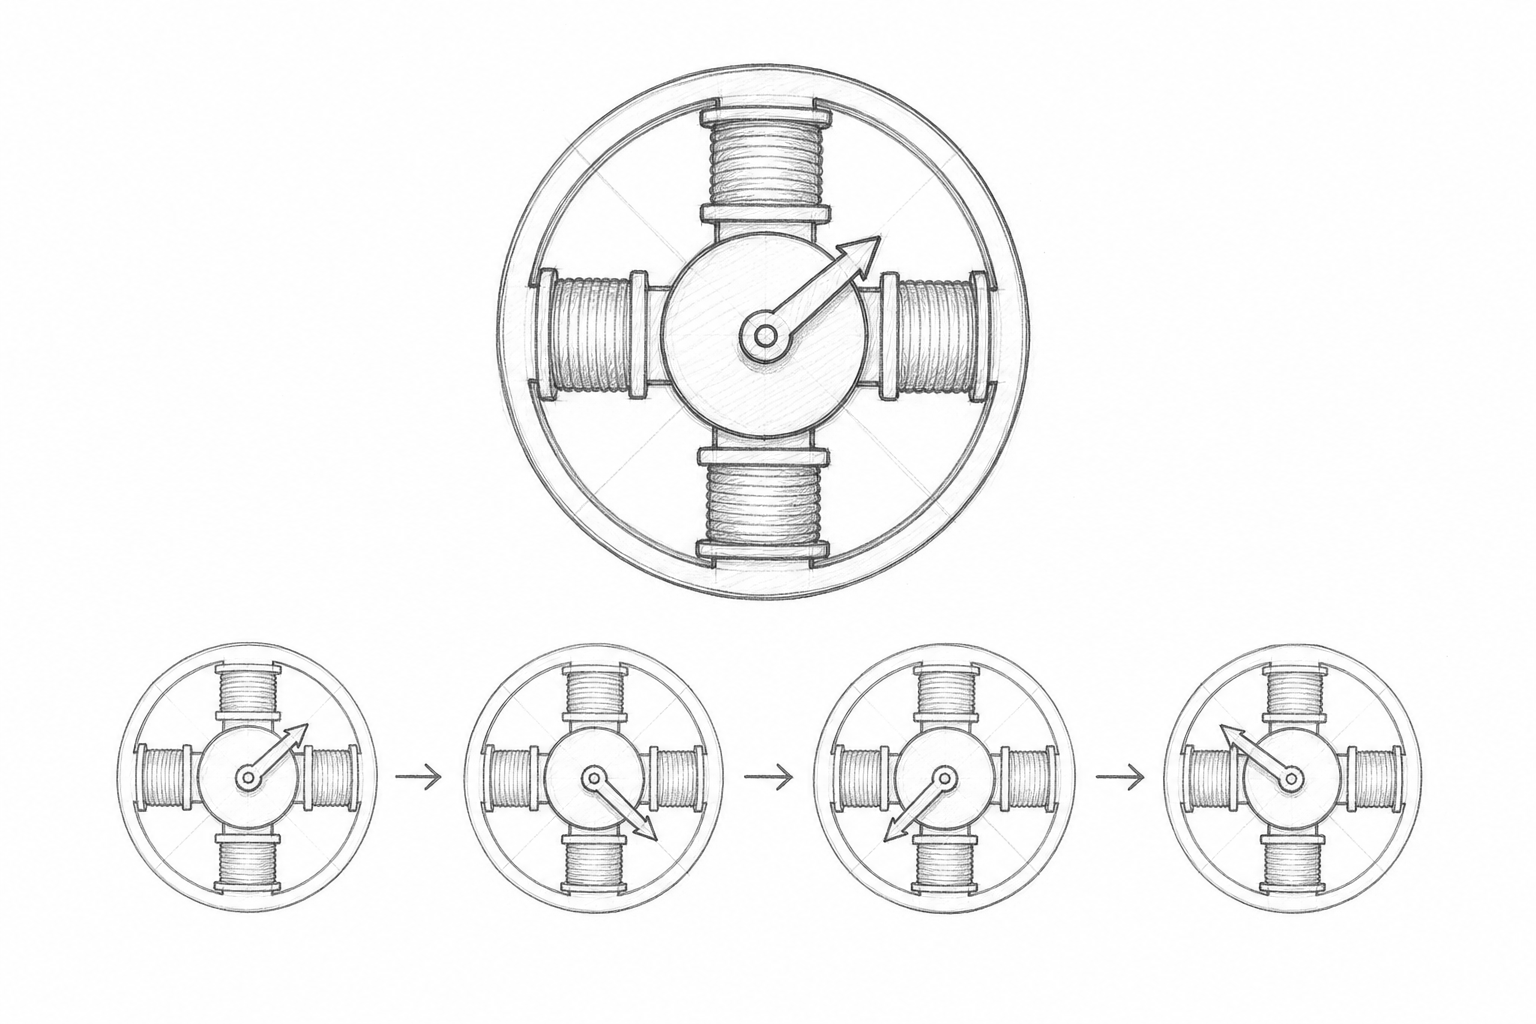
\includegraphics[width=0.96\linewidth,height=0.28\textheight,
 keepaspectratio]{047-logical-phase-wheel-pencil.png}

\small\textit{Alternative text: a graphite pencil concept drawing shows a
four-coil rotor and four successive pointer positions. It illustrates logical
sequence order only; it is not an electrical schematic or drive contract.}
\end{center}

The fixed half-step sequence is
\[
\texttt{0001,\ 0011,\ 0010,\ 0110,\ 0100,\ 1100,\ 1000,\ 1001}.
\]
Forward walks right through this list; reverse walks left. Each bit is a
logical intent only. It names neither a Mega pin nor a ULN2003 terminal.

\begin{tabularx}{\linewidth}{@{}c c c c X@{}}
\toprule
Index & Frame & Next forward & Next reverse & Prediction note\\
\midrule
0 & \texttt{0001} & \texttt{0011} & \texttt{1001} & \blankline\\[5pt]
2 & \texttt{0010} & \blankline & \blankline & \blankline\\[5pt]
4 & \texttt{0100} & \blankline & \blankline & \blankline\\[5pt]
6 & \texttt{1000} & \blankline & \blankline & \blankline\\
\bottomrule
\end{tabularx}

\newpage
\section{Bound rate and travel before acceptance}
\begin{center}
% ADK visual: pencil
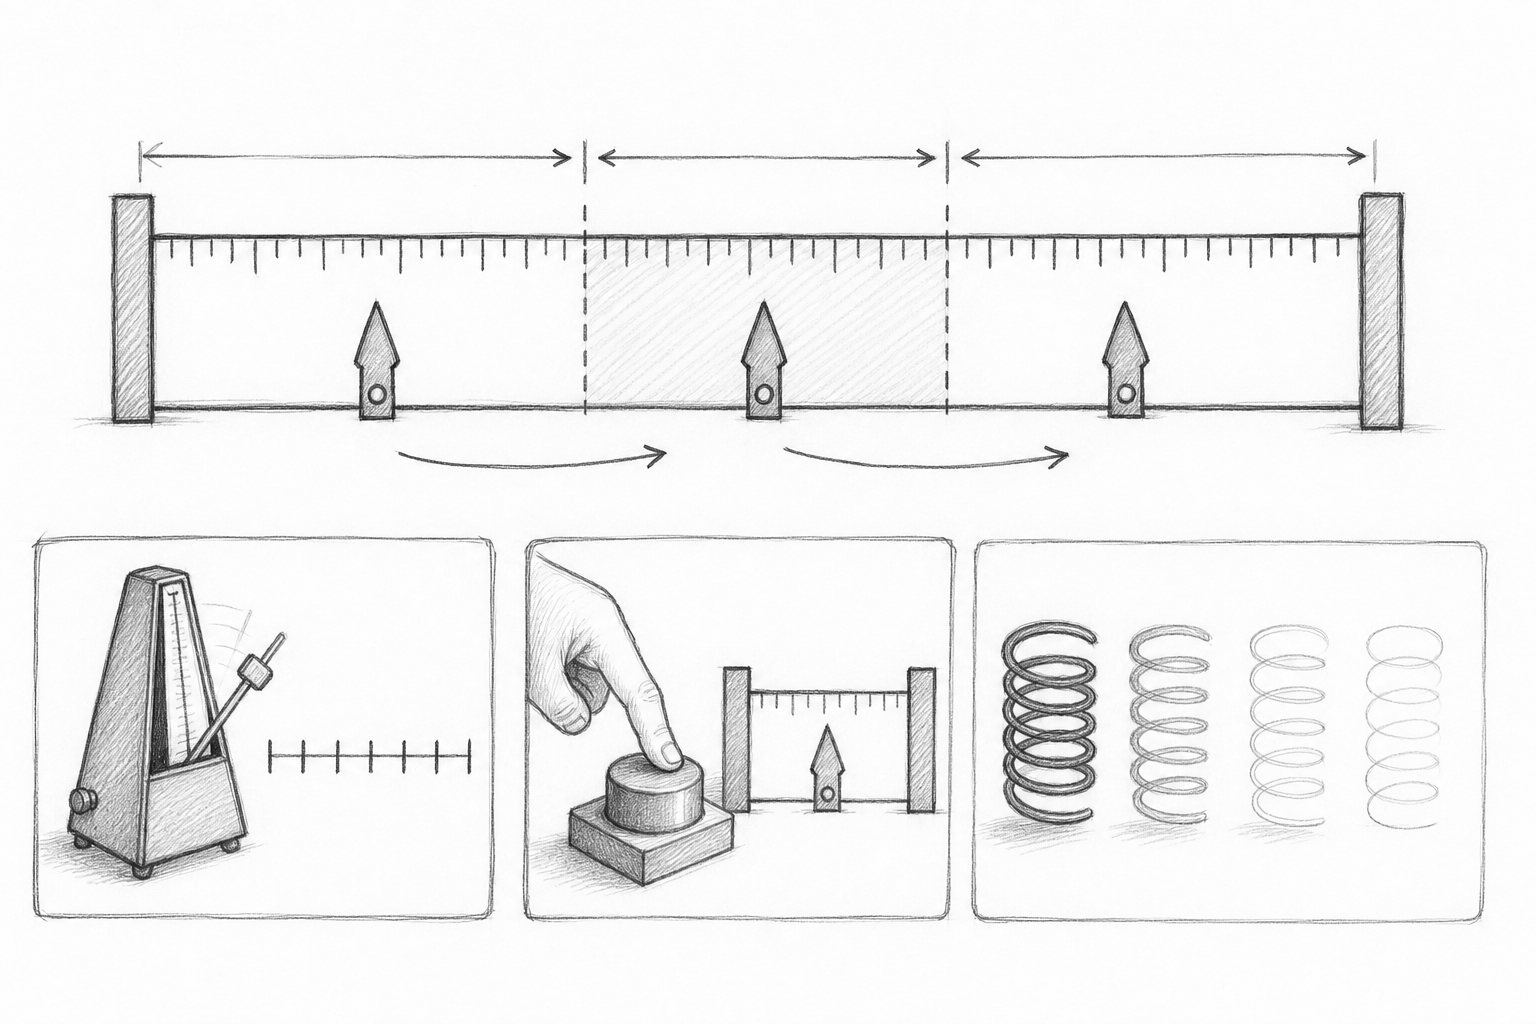
\includegraphics[width=0.97\linewidth,height=0.29\textheight,
 keepaspectratio]{047-bounded-motion-pencil.png}

\small\textit{Alternative text: a pencil storyboard shows a pointer confined
between two logical limits, caller-timed ticks, cancellation by a stop
gesture, and coil shapes fading to all-off intent.}
\end{center}

Configuration fixes the minimum and maximum interval, maximum command age,
minimum and maximum logical position, and whether a normally completed
command retains its last frame. Reject zero or wrap-unsafe durations,
reversed bounds, or a position range that widened arithmetic cannot update.

A moving command needs a nonzero ID, OK status, non-future issue time,
nonzero step count, interval inside the configured range, and a complete
endpoint inside the logical bounds. A stopped command requires zero steps.
Structural invalidity is rejected without changing accepted state.

\begin{tabularx}{\linewidth}{@{}X X X X@{}}
\toprule
Start & Direction / steps & Intended endpoint & Accept / reject\\
\midrule
\rule{0pt}{16pt}0 & forward / 8 & \blankline & \blankline\\[8pt]
7 & forward / 2 & \blankline & \blankline\\[8pt]
-7 & reverse / 1 & \blankline & \blankline\\
\bottomrule
\end{tabularx}

\subsection*{One-transition timing worksheet}
The first accepted moving command publishes all-off \texttt{0000}. Its first
deadline is
\(\mathit{issuedAt}+\mathit{stepInterval}\).
The first logical frame appears only on a call at or after that deadline. At
every due call, prepare exactly one next frame. If three deadlines elapsed,
three repeated calls catch up one frame at a time; the deadline cadence is
retained rather than stretched to ``now.''

\begin{tabularx}{\linewidth}{@{}r r r r X@{}}
\toprule
now (ms) & next due (ms) & before/at/after & frames advanced & next due\\
\midrule
9 & 10 & \blankline & \blankline & \blankline\\[7pt]
10 & 10 & \blankline & \blankline & \blankline\\[7pt]
35 & 20 & overdue & \blankline & \blankline\\
\bottomrule
\end{tabularx}

\newpage
\section{Use preview, then commit}
\texttt{preview()} is side-effect free. It prepares an opaque candidate bound
to one policy object and generation. \texttt{canCommit()} rejects a foreign,
stale, replayed, or already-used candidate. Only \texttt{commit()} publishes
the complete next snapshot. This seam lets Lesson 048 prove several candidate
policies admissible before changing any of them.

\begin{enumerate}
 \item Preview a valid command and copy the current snapshot. They must differ.
 \item Commit the candidate once. Copy the new snapshot.
 \item Try the same candidate again. It must be inadmissible and atomic.
 \item Prepare from a second policy. The first policy must reject that
       foreign candidate.
\end{enumerate}

\begin{tabularx}{\linewidth}{@{}l X X X@{}}
\toprule
Attempt & \texttt{canCommit} prediction & status & state unchanged / changed\\
\midrule
fresh owned preview & \blankline & \blankline & \blankline\\[8pt]
double commit & \blankline & \blankline & \blankline\\[8pt]
foreign owner & \blankline & \blankline & \blankline\\[8pt]
preview after reset & \blankline & \blankline & \blankline\\
\bottomrule
\end{tabularx}

\section{Distinguish completion, cancellation, stop, and fault}
\begin{tabularx}{\linewidth}{@{}l X X@{}}
\toprule
Event & Published result & What may happen next\\
\midrule
normal completion & \texttt{Complete}; final frame held only when configured
 & a forward-ID valid command may start\\
copied cancel & \texttt{Cancelled}; intent \texttt{0000}
 & a forward-ID valid command may start without reset\\
independent \texttt{stop()} & \texttt{Cancelled}; intent \texttt{0000}
 & a forward-ID valid command may start without reset\\
age expiry or time fault & \texttt{Fault}; intent \texttt{0000}
 & \texttt{reset()} is required before new motion\\
\texttt{reset()} & canonical \texttt{Inactive}; intent \texttt{0000}
 & remains initialized; a valid explicit command may start immediately\\
\bottomrule
\end{tabularx}

Cancellation dominates command meaning only after structural validity is
established and only for a live command. The independent stop is idempotent.
Neither path proves that current stopped flowing in physical coils.

\newpage
\section{Replay and inspect exact result cells}
Use
\href{https://github.com/spincyc/adk/blob/main/examples/Lesson047BoundedStepperSequence/Lesson047BoundedStepperSequence.ino}
{the Lesson 047 compile-only replay}. It stores copied command fields,
operation status, phase, disposition, direction, logical position, completed
steps, four-bit drive intent, deadline, and sequence status in named volatile
memory cells. Predict first; then record exact values.

\begin{tabularx}{\linewidth}{@{}c X X X X@{}}
\toprule
Frame & phase / disposition & position / completed & intent / next due & interpretation\\
\midrule
0 accept forward & \blankline & \blankline & \blankline & \blankline\\[7pt]
1 due step & \blankline & \blankline & \blankline & \blankline\\[7pt]
2 due step & \blankline & \blankline & \blankline & \blankline\\[7pt]
3 replace reverse & \blankline & \blankline & \blankline & \blankline\\[7pt]
4 due reverse & \blankline & \blankline & \blankline & \blankline\\[7pt]
5 copied cancel & \blankline & \blankline & \texttt{0000} / \blankline & \blankline\\[7pt]
6 restart forward & \blankline & \blankline & \blankline & \blankline\\[7pt]
7--8 finish & \blankline & \blankline & \blankline & \blankline\\[7pt]
9 independent stop & \blankline & \blankline & \texttt{0000} / none & \blankline\\
\bottomrule
\end{tabularx}

\lessonbox{\textbf{E0 observation path.} Named memory result cells are the
non-Serial evidence path for this pure replay. Mega compilation proves
packaging only. Do not run it on a powered board: the sketch owns no endpoint,
timer, interrupt, driver, supply, motor, stop switch, test point, or wiring.}

\section{Record measured resource evidence}
\begin{tabularx}{\linewidth}{@{}>{\bfseries}l r r X@{}}
\toprule
Artifact & Measured & Gate & Result / interpretation\\
\midrule
Lesson 047 Mega flash & 8,068 B & 16,384 B & \blankline\\
Lesson 047 static SRAM & 1,053 B & 2,048 B & \blankline\\
\texttt{BoundedStepperSequence} object & \blankline B & target 128 / hard 176 B & \blankline\\
host test executable & \blankline B & recorded host-size gate & \blankline\\
\bottomrule
\end{tabularx}

The first two measurements use the pinned Mega 2560 toolchain. Record the
tested commit and tool versions beside any newly measured blank. Size evidence
is not runtime, thermal, motion, or physical safe-state evidence.

\newpage
\small
\section{Diagnose the policy boundary}
\begin{tabularx}{\linewidth}{@{}l X@{}}
\toprule
Evidence & Interpretation\\
\midrule
same ID, changed payload & rejected mutation; accepted snapshot remains intact\\
forward modular ID while live & admissible replacement only if its full endpoint is bounded\\
ID regression or half-range ambiguity & rejected without mutation\\
several deadlines overdue & one transition per call; repeat calls to catch up\\
position exactly at configured limit & admissible endpoint, never evidence of a physical stop\\
expired command & \texttt{Fault}, all-off intent, reset required\\
cancel or independent stop & \texttt{Cancelled}, all-off intent; a later forward-ID command may start\\
hold-at-rest completion & logical frame may remain; no E2 hold-time or temperature claim\\
\bottomrule
\end{tabularx}

\section{Separate acquisition from safe state}
\begin{tabularx}{\linewidth}{@{}>{\bfseries}l X X@{}}
\toprule
Stage & Predict & Observe and interpret\\
\midrule
Acquire & initialize valid policy configuration & status cell: \blankline\\[8pt]
Act & commit one admitted logical transition & phase/position/intent: \blankline\\[8pt]
Safe state & cancel, stop, expiry, fault, or reset & exact intent:
\texttt{0000}; status: \blankline\\
\bottomrule
\end{tabularx}

Initialization acquires no hardware resource. All-off is a software intent,
not electrical high impedance or measured current removal. Resource
acquisition and safe-state evidence remain separate.

\section{Blank E2 promotion record}
\textbf{Leave every field blank at E0.} Compilation, simulation, retail
listings, and this workbook cannot fill a powered-motion acceptance cell.
\par\smallskip
\begin{tabularx}{\linewidth}{@{}>{\raggedright\arraybackslash}X X@{}}
\toprule
Required E2 field & Bench acceptance record\\
\midrule
exact motor / driver / board revisions and specimen markings & \shortblank\\[5pt]
authoritative formal schematic and mapped coil order & \shortblank\\[5pt]
separate supply rating, common reference, clamp path, measured current & \shortblank\\[5pt]
restraint, travel envelope, clearance, and guarded load & \shortblank\\[5pt]
independent stop and physical power-removal prediction / observation & \shortblank\\[5pt]
acquisition evidence separate from de-energized safe-state evidence & \shortblank\\[5pt]
maximum hold duration and winding / driver temperature evidence & \shortblank\\[5pt]
physical step count, direction, missed-step, and endpoint observations & \shortblank\\[5pt]
tool version / tested commit / reviewer / date & \shortblank\\
\bottomrule
\end{tabularx}

\section{Evidence links}
Open the
\href{https://github.com/spincyc/adk/blob/main/src/bounded_stepper_sequence.h}
{public interface},
\href{https://github.com/spincyc/adk/blob/main/tests/test_bounded_stepper_sequence.cpp}
{deterministic tests},
\href{https://github.com/spincyc/adk/blob/main/examples/Lesson047BoundedStepperSequence/Lesson047BoundedStepperSequence.ino}
{compile-only replay}, and
\href{https://github.com/spincyc/adk/blob/main/docs/design/LESSONS_046_048_KINETIC_SCULPTURE_PLAN.md}
{design plan with open gates}.
The searchable HTML lesson is the hardware-independent accessible route.
This untagged print edition makes no PDF/UA, powered-driver, physical-motion,
thermal, restraint, or stop-circuit acceptance claim.
\end{document}
